\documentclass[12pt,a4paper]{report}
\usepackage[utf8]{inputenc}
\usepackage[T1]{fontenc}
\usepackage{lmodern}
\usepackage{graphicx}
\usepackage{amsmath}
\usepackage{hyperref}
\usepackage[french]{babel}
\graphicspath{ {media/} }
\usepackage{csquotes}

%% Create the xx commande
\usepackage{soulutf8}  % Add the \hl command from soulutf8
\usepackage[dvipsnames]{xcolor}  % Add the color Apricot
\newcommand{\xx}[1]{%
  \begingroup
  \sethlcolor{Apricot}%
  \hl{xx #1 xx}%
  \endgroup
}

% To remove avec todo
\setlength {\marginparwidth }{2cm} % ajoute un peu de marges pour les todo
\usepackage{todonotes}
% To remove avec todo

\usepackage[natbib=true,backend=biber,style=apa]{biblatex}
\addbibresource{references.bib}


\title{
{Evolution of Cooperation in Collective Adaptative Systems}\\
{\large Sorbonne Université}\\
{
\includegraphics[width=\textwidth]{university.png}}
}
\author{Paul Ecoffet}
\date{\today}

\begin{document}

\maketitle

\chapter*{Abstract}
Abstract goes here

\chapter*{Dedication}
To mum and dad

\chapter*{Declaration}
I declare that..

\chapter*{Acknowledgements}
I want to thank...

\tableofcontents

\chapter{Introduction}
\input{chapters/01introduction}

\chapter{State of the Art}
\section{L'évolution de la coopération}

\subsection{L'évolution}
\label{ssec:evolution}

La coopération est un problème important en biologie évolutionnaire, qui étudie l'apparition et le maintien de traits morphologiques et comportementaux dans le vivant. D'après la théorie de la biologie évolutionnaire, chaque individu possède un certain nombres de caractéristiques qui peuvent être soit avantageuses soit désavantageuses pour l'individu dans son environnement comparé à ses pairs. Une caractéristique est dite avantageuse si elle permet à l'individu d'être plus adapté à son environnement que ses pairs, c'est-à-dire avoir une meilleure fitness. Cela signifie que l'individu a plus de capacité à survivre et à se reproduire s'il possède cette caractéristique comparé à ses pairs.

Si cette caractéristique est transmissible par reproduction, puisque l'individu se reproduit plus que les autres membres de la population, la caractéristique plus adaptée est de plus en plus fréquente dans la population. La descendance de cet individu est elle aussi plus adaptée que la descendance des autres individus, elle a donc un plus grand succès reproducteur. La descendance de la descendance de l'individu adapté est elle aussi plus adaptée comparé à celle de la descendance de la descendance des autres individus et ainsi de suite. La fréquence de la nouvelle caractéristique dans la population augmente au fil des générations au point que la caractéristique soit virtuellement dans toute la population. La caractéristique s'est fixée dans la population. C'est le mécanisme de sélection naturelle.

Ainsi, par sélection naturelle et reproduction, les caractéristiques les plus adaptées se propagent et se fixent dans les populations. Nous avons pris ici le cas simple d'une unique caractéristique, dans un environnement stationnaire. La fixation de caractéristiques peut être beaucoup plus complexe, parce que les caractéristiques qui définissent un individu peuvent avoir des interactions entre elles, ou bien l'environnement dans lequel évolue la population peut changer, soit de manière exogène au processus d'adaptation des individus, ou bien parce que le comportement des individus suite à la fixation de nouvelles caractéristiques viennent modifier celui-ci.

Nous avons ici présenté le premier ingrédient des mécanismes de l'évolution, la sélection. Le second élément est la variation. Nous avons précédemment postulé qu'un individu avait une caractéristique différente des autres membres de sa population. Comment peut-on avoir des variations de caractéristiques ? Précédemment, nous avons fait l'hypothèse implicite d'une transmission parfaite des caractéristiques du parent à la descendance. Faisons maintenant l'hypothèse explicite contraire : Il est possible que lors de la reproduction, il y ait une probabilité que la caractéristique transmise soit légèrement altérée. Cette altération peut avoir des conséquences marginales (la caractéristique est plus ou moins fortement exprimée), ou elle peut même avoir des conséquences importantes, comme changer complètement la nature de la caractéristique. Cette nouvelle version de la caractéristique peut être elle aussi adaptée ou non, et donc subir le même processus de sélection que décrit précédemment. 

Ainsi, le mécanisme de variation introduit de nouvelles caractéristiques dans la population, tandis que le processus de sélection vient conserver les caractéristiques les plus adaptées qui vont se fixer dans la population au détriment des moins adaptées qui vont elles s'éteindre. Ce processus, l'évolution, conduit un processus d'optimisation. À chaque génération, les caractéristiques qui maximisent la survie et la reproduction des individus se propagent.


\begin{verbatim}
ajouter exemples?
\end{verbatim}

\subsection{Le problème de la coopération}

En biologie de l'évolution, la coopération peut être définie comme le fait d'agir pour apporter un bénéfice à un autre individu. C'est un comportement très déroutant pour la biologie évolutionnaire. En effet, comment un tel comportement peut-il être adapté ? Un individu qui coopère dépense son temps et son énergie afin d'aider un autre individu. Il dépense des ressources pour augmenter la fitness, le succès reproducteur d'un autre. S'il est aisé de comprendre qu'être le bénéficiaire d'une coopération soit adapté et que ce comportement puisse être conservé par sélection naturelle, si tant est que ce serait transmissible, il est déroutant que la caractéristique \emph{d'être} coopérateur puisse être adapté. Il est difficile d'imaginer que cette caractéristique puisse être conservée par sélection naturelle. 

Pourtant, de nombreux cas de coopération sont observés dans le vivant. Tout d'abord, l'un des exemples les plus marquants pourrait être les insectes eusociaux, dont font partie les fourmis ou les abeilles. Pour ces espèces, les membres de colonies entières se coordonnent et travaillent ensemble afin de permettre le succès reproducteur de leurs reines. C'est un cas de coopération que nous développerons dans la section~\ref{ssec:altruism_kin}~\emph{\nameref{ssec:altruism_kin}}. Des comportements coopératifs sont aussi observés chez les gobemouches noirs, qui aident les autres gobemouches lorsqu'ils se font chassés par une chouette en attaquant collectivement le prédateur.  Ainsi, les gobemouches qui viennent aider la proie risquent leurs vies pour sauver celle d'un autre individu. Enfin, les humains sont de très grands coopérateurs. Ils possèdent des structures sociales complexes, produisent leurs ressources ensemble, les échangent, donnent à des organisations caritatives.


C'est comportements coopératifs sont comme dit précédemment très déroutant. Par exemple, il est aisé d'imaginer qu'un gobemouche noir qui n'attaque pas le prédateur d'un de ses partenaires pourrait avoir une meilleure fitness en ne mettant pas en danger sa vie. Comment expliquer que ces comportements n'ait pas été contre-sélectionnés ? Cette question est très fortement étudiée en biologie de l'évolution. De nombreux travaux ont identifié différents mécanismes qui permettrait de rendre les comportements de coopération viables. Ces mécanismes sont détaillés dans les prochaines sections.



\subsection{L'altruisme et l'apparentement}
\label{ssec:altruism_kin}

Une première explication des comportements coopératifs est la sélection de parentèle \citep{Hamilton1964}. Les explications de l'évolution donnés dans la section~\ref{ssec:evolution}~\emph{\nameref{ssec:evolution}} étaient centrées sur l'individu. Cependant, la propagation de caractéristiques est plus complexe que cela. L'individu n'est qu'un véhicule transportant la caractéristique, et celle-ci . Le support de cette caractéristique dans le vivant est le gène. Le gène code cette caractéristique. Le support même. \todo{compléter} 

Ainsi, il peut être rentable pour un individu d'aider un de ses apparentés, si le bénéfices $b$ pour le bénéficiaires pondérées par le degré d'apparentement $r$ surpasse les coûts engagés par l'acteur $c$, alors le comportement altruistique est stable. C'est la règle d'Hamilton définie dans l'équation~\ref{eq:hamiltonrule}.

\begin{equation}
r \times b > c \label{eq:hamiltonrule}
\end{equation}


Dans ce cas là, c'est aider des parties de soi plutôt que d'aider qqun d'autre. Cette implémentation de la coopération est mise en places chez les insectes eusociaux tel que les fourmis ou les abeilles, où le degré d'apparentement entre les individus d'une même colonie est de 75\%, ou bien entre les cellules d'organismes multicellulaires, où le niveau d'apparentement est ici de 100\%.

Cependant, cela permet de comprendre qu'un sous-ensemble des comportements observés dans le vivant. Comment les comportements de coopération entre individus d'espèces différentes ont pu évoluer ? De même, comment les comportements entre individus d'une même espèce mais non-apparentés, comme on l'observe chez l'Humain ou chez les chauves-souris vampires par exemple peuvent se développer.

\subsection{La réciprocité}

Un gène ne peut être conservée au cours de l'évolution uniquement si ce gène déploie un phénotype plus adapté que le phénotype de ses concurrents pour sa reproduction. Comme vu dans la section~\ref{ssec:altruism_kin}~\emph{\nameref{ssec:altruism_kin}}, cela peut se faire de manière indirecte, ce qui permet d'expliquer les comportements de coopération entre apparentés. Dans le cas de coopération entre non-apparentés, c'est donc que le comportement de coopération exprimé par le gène d'un acteur apporte bien un bénéfice à cet acteur lui-même. En effet, sans sélection de parentèle, l'expression du gène ne possède aucun moyen de déterminer si le bénéficiaire de la coopération possède lui aussi le même exemplaire de ce gène. Quand bien même le bénéficiaire posséderait les mêmes expressions phénotypiques que l'acteur, cela ne garantit pas la propagation du gène responsable pour ce comportement. \todo{green beard \cite{Dawkins1976}} Ainsi, un gène qui code pour un comportement coopératif, c'est-à-dire qui code un comportement aillant un coût pour l'acteur et un bénéfice pour le bénéficiaire, doit forcément apporter un bénéfice comparé à ses concurrents.

C'est le cas si le comportement coopératif de l'acteur entraîne un changement de comportement sur le bénéficiaire, comme le propose \citet{Trivers1971}. Ainsi, il est intéressant d'agir de manière coopérative avec un individu qui le sera lui aussi avec nous en retour. C'est la coopération conditionnelle ou la réciprocité. Cette réciprocité peut être soit positive, c'est à dire que le bénéficiaire coopère avec l'acteur en réponse à la coopération ; soit négative, le bénéficiaire punit l'acteur si celui-ci ne coopère pas. Dans les deux cas, il est dans l'intérêt de l'acteur de coopérer, puisque cela maximise son gain en vu de la réaction du bénéficiaire. Notons cependant qu'agir de manière coopérative n'a de sens ici uniquement si cela a un effet sur le comportement du bénéficiaire. Si le bénéficiaire aurait de toute façon aider l'acteur après coût, ou bien si le bénéficiaire lui aurait de toute façon causer dommage, alors l'acteur n'a aucun intérêt à coopérer en faveur du bénéficiaire. C'est en cela qu'il y a réciprocité. Les comportements de réciprocité peuvent être implémenté très facilement et sont particulièrement robuste, comme l'a montré \citet{Axelrod1981}. Ainsi, dans le cadre d'une situation de coopération modélisable comme un dilemme du prisonnier, avec interactions répétées, le comportement de tit-for-tat est une stratégie de réciprocité extrêmement robuste. De même, les comportements de punition chez les poissons nettoyeurs avec leurs clients \citep{bsharyxx}. Les comportements tit-for-tat se retrouvent aussi avec les gobemouches noirs \citep{Krams2008}, qui ne viennent défendre que les gobemouches noirs qui les ont déjà défendu auparavant, mais jamais ceux qui ne sont jamais venu les aider alors qu'ils en avaient besoin.

Il y a ainsi deux types de réciprocité directe: Le Partner Fidelity Feedback et le Partner Choice \citep{Sachs2004}.

\subsection{Le choix du partenaire et les marchés biologiques}

\xx{Parler d'opportunités de coopération !!!}

Parmi les implémentations de la coopération par réciprocité, le choix du partenaire semble être apparu de nombreuses fois et être un mécanisme particulièrement efficace. Dans l'espèce Humaine, il joue un rôle prépondérant dans le maintien des comportements de coopération. Le choix du partenaire permet l'apparition et le maintient de la coopération. Pour le comprendre, ne nous centrons plus sur l'acteur de la coopération, mais le bénéficiaire. Dans une tâche collective, il est toujours pertinent pour le bénéficiaire de la tâche collective de se mettre avec le meilleur acteur possible, c'est-à-dire l'acteur qui lui permettra d'obtenir le plus gros gain. Puisque pour réaliser la tâche, qui est \emph{collective}, l'acteur a aussi besoin du bénéficiaire, il est alors dans l'intérêt des acteurs d'être le plus coopératif possible afin d'être choisi par un bénéficiaire. Ainsi, il y a une pression a être coopératif afin d'être choisi par un bénéficiaire. Cette pression est d'autant plus forte si le nombre d'acteurs est particulièrement grand par rapport au nombre de bénéficiaire. Il y a un effet de marché \citep{Noe1994}.

Imaginons maintenant une population d'individus qui cherche à être avec le meilleur partenaire possible, et que tous les individus présents dans cette population sont égoïstes. Dans cette population apparaît un mutant qui coopère plus que les autres. Ce mutant va être particulièrement recherché par les autres individus de la population. Il va donc interagir beaucoup et obtenir de nombreux gains. De la même manière, puisque de nombreux individus vont vouloir coopérer avec lui, il va pouvoir être sélectif. Il va pouvoir refuser les interactions avec les moins efficaces pour choisir les interactions avec les plus performants. Il y a donc un assortative matching qui se met en place. Les individus les plus performants qui interagissent ensemble vont recevoir de très nombreux bénéfices de leurs interactions. Ces bénéfices ont un impact positif sur leur fitness et ils vont se propager dans la population. Le fait d'être coopératif va se fixer dans la population et tous les individus seront des coopérateurs.

Le choix du partenaire

Ces mécanismes de choix du partenaire se retrouvent dans la nature. C'est ainsi eux qu'on observe dans les mutualismes inter-spécifique chez les cleaners fishes et leurs clients \citep{Bshary2002b} \todo{détailler} ou bien chez les mutualismes legumes-rhizobium \todo{source + détail}.


partner switching

\cite{Aktipis2011}


\begin{verbatim}
Choisir un partenaire pour le gain qu'il nous apporte, non pas pour l'aider lui. crée une boucle
- grooming
- vampire bats
- cleaner/client
\end{verbatim}

\subsection{Pourquoi la coopération n'est pas partout ?}

Bien que nous nous demandions en début de ce chapitre comment la coopération pourrait évoluer, après l'étude des différents mécanismes qui puissent l'implémenter, c'est maintenant la question contraire qui apparaît. Comment se fait-il que la coopération entre non-apparentés soit en fait si rare dans la nature ? En effet \xx{exemple de pas coopération même si c'est tendu}, et pourtant le choix du partenaire est un mécanisme particulièrement puissant chez l'Homme \todo{cite}. 

Quels sont les paramètres qui pourrait empêcher l'apparition de réciprocité ?

Tout d'abord, il faut souligner le problème du bootstrapping. S'il est aisé de comprendre comment les mécanismes de réciprocité peuvent maintenir les comportements de coopération, il est en fait plus compliqué d'expliquer comment ce mécanisme peut apparaître de lui-même. En effet, la réciprocité -- tant la Partner Fidelity Feedback et le Partner Choice -- requiert.

bootstrapping
Dans ce cas, pourquoi la coop n'est pas partout? Qu'est-ce qui la bloque ?
Objectif de la thèse : capturer le pourquoi la coop c'est difficile


%%%%%%%%%%%%%%%
%%%%%%%%%%%%%%%

\section{Modèles et méthodes}

\subsection{Les modèles analytiques}

Théorie des jeux évolutionnaire

\subsection{Les modèles agents centrés}

McNamara, Aktipis(?)

\subsection{La robotique évolutionniste}

importance des problèmes de coordination et mécanistes.
Intéressant d'avoir des robots capables de coop

\subsection{Le mapping génotypique-phénotypique}

%%%%%%%%%%%%%%
%%%%%%%%%%%%%%

\section{Objectif de la thèse}

\begin{verbatim}
    
comprendre pourquoi la coopération bloque, pourquoi c'est difficile à obtenir
- Utilisation de modèles agents centrés et robotiques pour capturer les difficultés présentes et que ne capturent pas les autres modèles
-> Contraintes de coordinations, d'accès au ressources, de densité, de navigation
\end{verbatim}



\chapter{Nothing better to do? Environment quality and the evolution of cooperation by partner choice}
Several mechanisms have been identified to explain the evolution of cooperation among non-kin \citep{Trivers1971, MaynardSmith1974, Axelrod1981}, including positive reciprocity \cite{Trivers1971, Axelrod1981, Andre2007}, punishment \cite{Bshary2005, Raihani2012} or partner choice \cite{Eshel1982, Bull1991, West2007, Schino2017}. Among these mechanisms, partner choice has been considered over the last twenty years as having probably played a particularly important role \cite{Baumard2013a, +ref}. When individuals can choose among several different partners, which they can compare and compete against each other as in an economic market, this generates a selection pressure to cooperate more, to appear as a good partner and attract others' cooperation \cite{Noe1994}.

The effects of partner choice have been well documented in a large number of biological systems. For example, in the interaction between cleaner fishes and their clients the law of supply and demand determines the way in which the added value of the interaction is shared, in accordance with market principles \cite{Bshary2006}. When cleaners are rare, clients tolerate cheating on their part, while they become more picky when cleaners are numerous. The effects of partner choice have also been documented in primate grooming behavior in two meta-analyses, showing that female primates groom preferentially those that groom them most and that a positive relation exists between grooming and agonistic support \citep{Schino2007, Schino2008}. In vervet monkeys, individuals groom others in exchange for access to food and they do so for longer periods when fewer partners are available \cite{Fruteau2009}. Beyond cooperation, partner choice also plays a decisive role in mating, leading to the evolution of secondary sexual caracteristics and nuptial gifts, and/or to assortative matching (refs xxxTODOxxx \cite{Zahavi1975, xxTerrain}. Lastly, the effects of partner choice have also been documented in humans where it has been shown that the need to attract social partners is a major driver of cooperation \citep{Barclay2007a, Barclay2015, Barclay2016, Debove2015b,  Andre2011, Baumard2013a}.

% xx \cite{Clutton-brock2009} qui discute plein de cas de réciprocité qui pourrait n'être qu'en fait manipulations et mutualismes


There are, however, a number of biological situations in which one would typically expect partner choice to play an important role, but where no such effect has ever been demonstrated. These include most intraspecific collective actions in non-human animals. This is particularly salient in collective hunts such as collobus hunting in chimpanzees, or pack hunting in carnivores. No empirical evidence in these species suggests that individuals cooperate for reasons related to partner choice, either to attract partners or to be accepted by them in their hunts. On the contrary, the majority of available data are consistent with the more parcimonious explanation that individuals are simply doing what is in their immediate best interest at any given time \cite{Packer1986,Packer1988a, Melis2008, Melis2011}. In particular, if cooperation in collective hunts was driven in part by the need to appear as a good partner, individuals would be expected to  willingly share the product of their hunts in a way that depends on everyone's actual engagement, to encourage participation in other hunts in the future. However, such voluntary and conditional sharing has never been documented in animal collective hunts \cite{Melis2011}. In evolutionary terms, therefore, collective hunting in these species is most likely an instance of \textit{byproduct} cooperation, rather than an instance of reciprocal cooperation based on partner choice.

Yet several models on the evolution of cooperation by  partner choice suggest that cooperation should evolve in these situations \cite{McNamara2008, Aktipis2011, Barclay2011, Campenni2014}. And, in humans, behaviours in collective actions are driven by the need to appear as a good partner, especially when it comes to sharing the benefits of cooperation (refs Alvard xx \cite{Baumard2013a}). One may therefore wonder why the same effects did not produce the same consequences in other species.

Such a lack of observation could always be the consequence of methodological difficulty in empirically proving the existence of partner choice. However, we would like to suggest an alternative here, namely that there is in fact a strong constraint impeding partner choice in a large number of situations in animals.

Partner choice requires that individuals can compare and choose among several opportunities for cooperation. In some cases, \textit{partners} themselves constitute opportunities for cooperation and partner choice then only requires that partners are many and accessible. This is the case, for instance, in mating markets, or in most instances of interspecific mutualism. In other cases, however, finding an opportunity for cooperation requires more than just finding a partner. This is what happens when cooperation consists of several individuals working together to exploit environmental resources. In this case, a cooperation opportunity requires both a partner(s) and a resource, which imposes an additional constraint limiting the scope of partner choice. When resources are scarce, there are always few options to compare, and partner choice cannot operate. This could explain the lack of cooperation, beyond by-product cooperation, in many instances of collective actions in the wild despite the availability of potential partners.

In this article, we aim to test this idea using agent-based simulations. To do this, we simulate the evolution of agents placed in an environment containing resources that can be exploited collectively. We show that, in a low-resource environment, and even if there are plenty of partners, partner choice is not able to drive the evolution of cooperation as individuals cannot pit the few cooperation opportunities against each other. What is more, we also show that the number of potential partners actually has a negative effect on the evolution of cooperation when patches are scarce. When there are too many potential partners relative to the amount of patches available, there are always too many individuals on any given resource as individuals have nothing else to do anyway. Hence, there is no point in trying to attract partners but on the contrary there are benefits in trying to limit their number. We therefore show that partner choice is only effective when the number of available partners lies within a precise range of values, all the narrower as the availability of patches is low.

We believe that this constraint plays a central role in explaining that, in many species, although individuals do participate in collective actions, sometimes finely coordinating their behaviour with that of others, individuals do not actually seek to cooperate beyond what is in their immediate personal interest. On the contrary, thanks to its cognitive capacities, the human species is able to extract resources from a greater variety of situations. As a result, we actually live in an environment that is much richer in resources than other species. Hence we can compare and compete a greater diversity of opportunities for cooperation against one another, and we are thus forced to cooperate more intensively to attract partners.


\section{Methods}

We consider a population of $N_T$ individuals living in an environment consisting of $\omega$ different patches on which resources are located. Every generation of the simulations is constituted of $T$ time steps during which individuals gather payoff units. At the end of these $T$ time steps, individuals reproduce in proportion to their total payoff, and die. During a time step, every individual is considered one by one in a random order. When her turn comes, an individual evaluates each of the $\omega$ patches of the environment, including the patch where she is currently located, assigns each a score, and then moves toward the patch with the highest score, or stays on her current patch if that's the one with the highest score. Once every individual has taken this decision, individuals express their cooperation strategy on their local patch, and they collect a payoff that depends on their own and their partners' cooperation strategy. Patches can disappear every time step, with a probability $d$, and are then immediately replaced by an empty patch.

xx La taille de la population totale $N$ est toujours constante quelque soit le nombre d'individus présents dans l'environnement $N_T$ afin d'avoir le même nombre d'évaluations d'individus dans toutes les conditions. Pour $N_T < N$, $N_E = \lceil N_T / N \rceil$ environnements sont créés. Les individus sont répartis aléatoirement dans ces environnements afin que chaque environnement comporte $N_T$ individus. Pour le dernier environnement à compléter, s'il n'y a pas $N_T$ individus encore disponibles, alors des individus tirés d'autres environnements sont inclus dans l'environnement pour le compléter. Les gains obtenus par ces individus dans cet environnement ne sont pas considérés pour le calcul de leurs fitnesses.

\subsection{The decision-making mechanisms}

The individuals' strategy in this environment consists of two separate decisions.

On the one hand, the individual must evaluate the different patches available and assign a score to each. This decision is made by an artificial neural network, called the "patch ranking" network. For each patch, this neural network has the following input information: (i) the number of other individuals already present on the patch, (ii) the average level of cooperation expressed by these individuals in the last time step, (iii) the level of cooperation that the focal individual would express should he join this patch, and (iv) a binary that indicates whether or not the individual would have to move in space in order to join this patch (i.e. this binary distinguishes the patch where the individual is currently located from all other patches).

(xx En supplementaries plutôt ? C'est vraiment du détail d'implem…

Pour (i), (ii) and (iii), leurs valeurs sont séparées en décimales et unités et envoyées dans des entrées différentes pour permettre au contrôleur de distinguer facilement de faible variations.
)

On the other hand, the individual must decide on a level of cooperation once she is on a patch. This decision is made by another artificial neuron network called the ``cooperation'' network (plus some phenotypic variability, see below). As an input, this neural network only has the number of other individuals present on the same patch as the focal. This entails that we assume that the agent cannot modulate her cooperation level in function of others' cooperation level. This assumption is meant to exclude the possibility that partner control strategies may evolve, and allows us to focus only on the effect of partner choice.

The connection weights of both networks constitute the genome of each agent. They evolve by natural selection as exposed in the section \ref{sec:evolutionaryalgo}.


\subsubsection{Phenotypic variability of cooperation}\label{ssec:phenotypic_var}

As is now well established in the litterature, selective pressures in favor of any form of conditional cooperation, and therefore in particular in favor of partner choice, stem from the presence of some variability in partners’ cooperative behavior (see \cite{McNamara2010c} for a review of this idea). In order to capture the effect of variability in the simplest possible way, here we consider the effect of phenotypic variance in the expression of individuals' genes. At each generation of our simulations, each individual is subject to the effect of a \emph{phenotypic noise} that modifies her cooperation level. If $x_i^g$ is the cooperation level chosen by the genes of an individual (i.e. decided by her cooperation network), then the actual cooperation level player by the individual is $x = x_i^g + \epsilon$, where $\epsilon$ is drawn ramdomly as follows. The interval $[-1, 1]$ is uniformly split in $N_T$ values, and every individual gets one value of $\epsilon$ chosen among these $N_T$ values without replacement.


\subsection{The payoff function}

Each individual $i$ present on a patch invests a given amount $x_i$ into cooperation --where $x_i$ is decided by the individual's cooperation network. Individuals present on the same patch play a modified version of the n-player prisoner's dilemma. Consider a focal individual $i$ playing $x_i$, in a patch on which there are $n-1$ other individuals whose average level of cooperation is $\bar{x}_{-i}$ . The payoff of individual $i$ is given by

\begin{equation}
P(x_i, \bar{x}_{-i}, n) = F(n)  \times  \left[ a x_{i} +  b  \bar{x}_{-i} - \frac{1}{2}  x_i^2\right]
\end{equation}
xx où $a$ représente le bénéfice propre de l'agent et $b$ represents the social benefit of others' cooperation, and the function $F(n)$ is meant to capture the fact that there is an optimal number of individuals exploiting a patch and is given by

\begin{equation}
F(n) = e^{ - \left( {n - \hat{n} } \right)^2  / (2\sigma^2) } \label{eq:friction}
\end{equation}where $\hat{n}$ is the optimal number of individuals per patch and $\sigma$ measures the strength of the penalty that stem from being a submoptimal number of individuals on the same patch.

This payoff function has been chosen in such a way that, in the absence of partner choice, the evolutionarily stable strategy is always to invest the individually optimal investment (i.e. $x_{ESS} = a$), whereas the ``socially optimal'' cooperation, that is the level of cooperation that would maximise the average payoff of individuals on the patch, is to invest $\hat{x} = a + b$.


% \begin{figure}[htbp]
%     \centering
%     \includegraphics[width=\linewidth]{lions/methods/payoff.pdf}
%     \caption{Variation of the payoff for the focal player according to its partner investment strategy for $n=2$}
%     \label{fig:payoff}
% \end{figure}

% Note: pourquoi social optimum quand P(x, x)? Nécessite une explication qui ne va pas de soi (?).



\subsection{The evolutionary algorithm}\label{sec:evolutionaryalgo}

Each individual has a genome composed of the weights of its two neural networks, which makes a total of 84 genes $g = (g_{1}, \ldots, g_{84})$ with $ g_{i} \in ]-10, 10[$. We consider a population of fixed size $N$. The first generation is composed of $N$ individuals with random genes for the neural network weights, drawn uniformly in $]-1, 1[$. We then use a fitness proportionate evolutionary algorithm to simulate  evolution.  After the $T$ time steps of a generation have taken place, individuals all reproduce and die. A new population of $N$ individuals is built out of the previous generation by sampling randomly among the $N$ parents in proportion to their cumulated payoff, according to a Wright-Fisher process.

A mutation operator is applied on each offspring. Every gene of every offspring has a probability $\mu$ to mutate and a probability $1-\mu$ to stay unchanged. If a gene $g_i$, with value $v_i$, mutates, it has a probability $0.9$ to mutate according a normal distribution and thus reach a new value sampled in $\mathcal{N}(v_i, 0.1)$ and a probability $0.1$ to mutate according to a uniform distribution and thus reach a new value sampled in $\mathcal{U}(]b_{min}, b_{max}[)$.

The evolutionary algorithm is run for $G$ generations.


\begin{table}
    \centering
    \begin{tabular}{clc}
        \hline
        \textbf{Parameter} & \textbf{Description} & \textbf{Value}  \\
        \hline
        \textbf{Environment} & & \\
        $N$ & Population size & $100$ \\
        $d$ & Probability of disappearance of partches, per time step & $1/1\ 000$ \\
        $T$ & Number of timesteps per generation & $1\ 000$ \\
        $c_{m}$ & Cost of moving to another patch & $0$ \\
        $N_T$ & Number of individuals in the local environment & var \\

        \textbf{Payoff } & & \\
        $a$ & Immediate personal benefit of cooperation & $5$ \\
        $b$ & Social benefit of cooperation & $5$ \\
        $\hat{n}$ & Optimal number of individuals per patch & var \\
        $\sigma$ & Tolerance to variations in the number of individuals per patch & var \\
        \textbf{Evolution} & & \\
        $G$ & Number of generations & $1\ 500$ \\
        $\mu$ & Probability of mutation per gene per generation & $0.01$ \\
        \hline

    \end{tabular}
    \caption{Parameters of the simulation}
    \label{tab:parameters}
\end{table}


\section{Results}

\subsection{Cooperation cannot evolve when patches are scarce}

We simulated the evolution of a population of $N_T=100$ individuals for $G=1500$ generations, for different values of the number of resource patches $\omega$, but always in a situation where the optimal number of individuals per patch was $\hat{n}=2$. Cooperation only evolved when patches were more abundant than a threshold (Fig.~\ref{fig:varyingopp}, a). This can be understood as follows. When resource patches are few, precisely when $\omega < \frac{N_T}{\hat{n}}$, individuals have little cooperation opportunities and there is therefore always more individuals per patch than what would be optimal (in this case, the optimal number of individuals per patch is $\hat{n}=2$). As a result, additional individuals joining a patch are more of a nuisance than a benefit, and there is therefore no benefit in trying to attract partners by appearing cooperative.

\begin{figure}[tb]
    \centering
    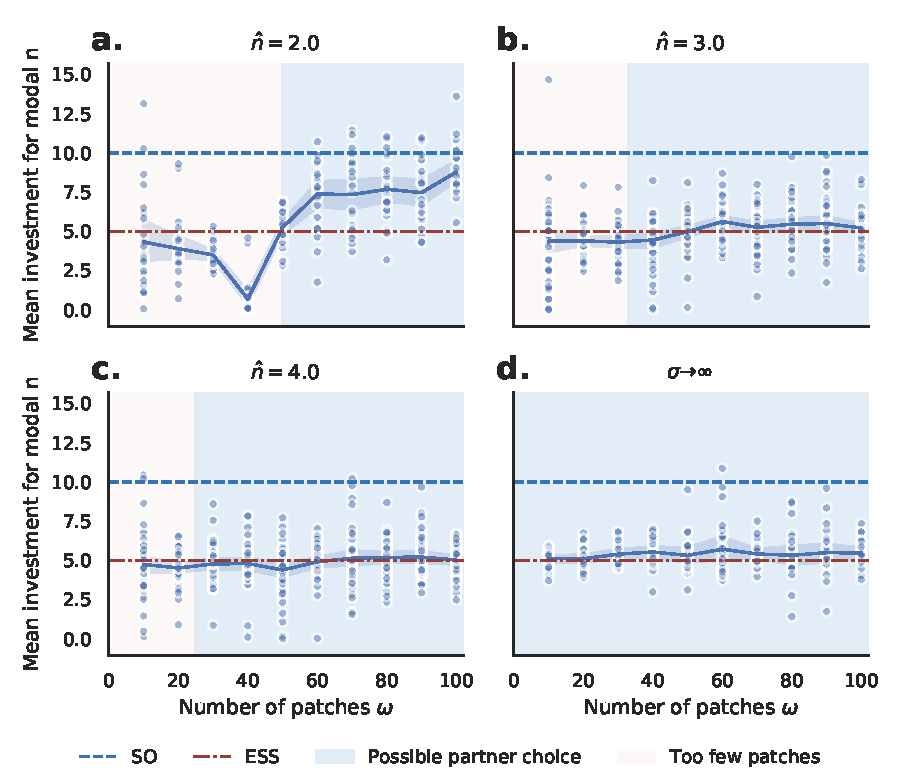
\includegraphics[width=\columnwidth]{lions/results/byprod/varopp_hatn_1.pdf}
    \caption{Mean investment in simulation for different number of opportunities $\omega$ and a fixed population of $N_T=100$ individuals. Results after $1\,500$ generations. \textbf{a.}~When $\hat{n} = 2$ Cooperation evolves when $\omega \geq 50$. \textbf{b-c.}~For $\hat{n} \geq 3$, cooperative behaviours never evolve. \textbf{d.}~When $\sigma \to \infty$, there is no pressure for agent to attract partners and cooperative behaviours never evolve.}
    %\par \small
    %When there is not enough patches to host all the agents in the environment, agents have no outside options. Therefore, they have no better choice than staying with their current partners.
    %If there is enough patches, agents can easily find available opportunities. Therefore, they have plenty of outside options. Partners must invest sufficiently enough to satisfy the agent.

    \label{fig:varyingopp}
\end{figure}


We then simulated the evolution of cooperation in situations where the optimal number of individuals per patch, $\hat{n}$, was larger (Fig. \ref{fig:varyingopp}, b-c). Overall, the outcome was even less favorable to cooperation. This may seem paradoxical but can be understood as a consequence of the law of large numbers. When the number of individuals per patch is large, whether it is greater or less than $\hat{n}$, the effect of each individual on the average quality of her patch is very small anyway. There is therefore little value for an individual to invest in cooperation to try and attract partners.

Finally, we performed the same simulations in the case where the number of individuals per patch is neutral ($\sigma \rightarrow \infty$, Fig. \ref{fig:varyingopp}, d). Cooperation did not evolve either and this can be understood also because there cannot be any benefit in attracting partners when the number of individuals per patch does not matter.

Overall, the evolution of cooperation by partner choice can only take place in the restricted conditions where (i) there is an optimal number of individuals per resource patch, (ii) this optimal number is low, and (ii) the number of resource patches in the environment is large.


\subsection{Cooperation cannot evolve when there are too many partners around}

In a second step, we simulated again the evolution of a population of $N=100$ individuals for $G=1500$ generations in a situation where the optimal number of individuals per patch was $\hat{n}=2$, but this time we held the number of patches constant, $\omega = 20$, while varying the actual number of individuals, $N_T$, present together in the environment.

In this case, cooperation only evolved when the number of individuals in the environment was intermediate. This can be understood as follows. When the number of individuals in the environment, $N_T$, is too close to the number of individuals, $\hat{n}$, that are needed to exploit at least one patch --or even more so when $N_T < \hat{n}$ , then the number of available partners is limiting. As a result, the actual number of cooperation opportunities from which individuals can choose is very low, partner choice is thus a weak force, and the benefit of investing into cooperation is low. On the other hand, when the number of individuals in the environment, $N_T$ is larger than the total number of individuals that can be accomodated on the available patches, that is when $N_T > \hat{n} \omega$, the number of available patches is limiting. In this case we find the result described above (Fig. \ref{fig:gridtol1}, a). The problem is rather that there are always too many individuals on each patch than too few and partner choice is also a weak force. There is, therefore, a range of intermediate population densities, neither too low nor too high, for which cooperation can evolve.

We then performed the same simulations again, but with more patches available in the environment (i.e. for larger $\omega$, Fig. \ref{fig:gridtol1}, b, c). We observed that the range of population densities for which cooperation could evolve was then broader. This can again be understood in the above framework. On one hand, the lower boundary of population density, $N_T \approx \hat{n}$, below which the number of individuals is a limiting factor, is unaffected by the amount of patches available.  On the other hand, the upper boundary of population density, $N_T > \hat{n}\omega$, above which the number of patches is a limiting factor, increases with the amount of patches, $\omega$ . As a result, the width of the range of population densities where partner choice is effective increases.

\begin{figure*}
    \centering
    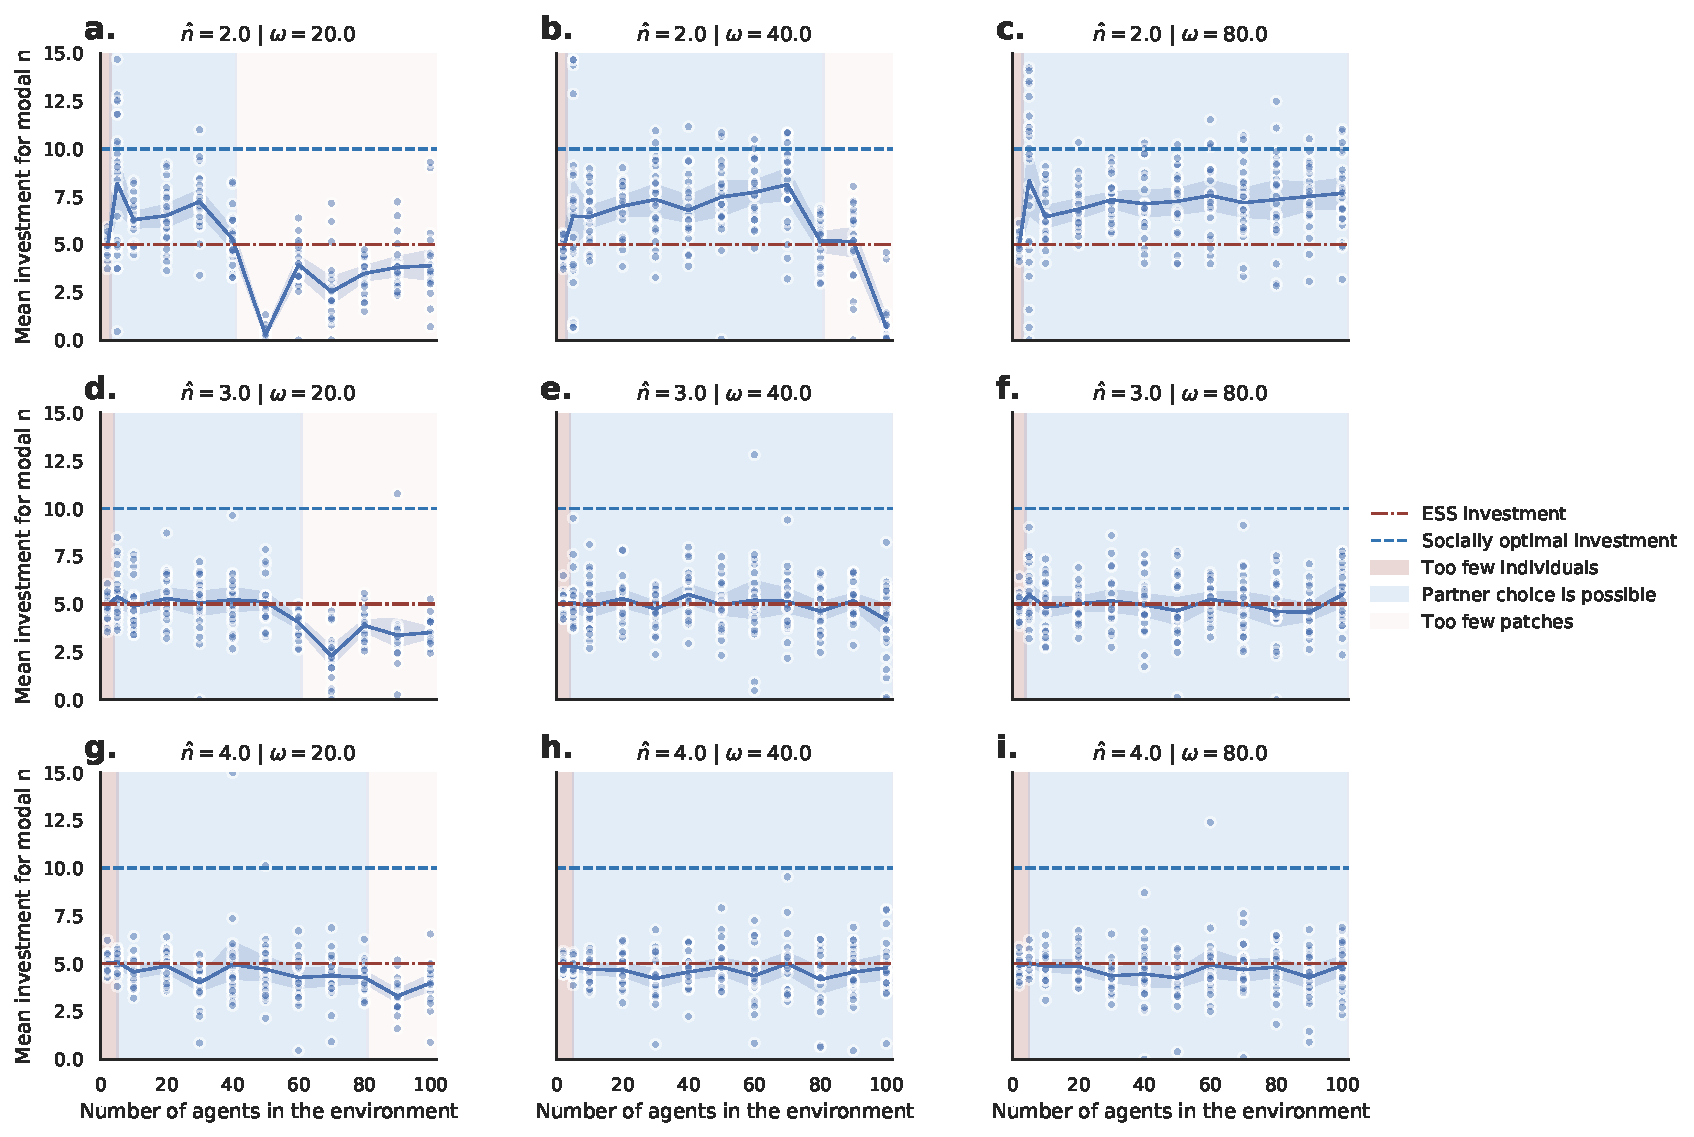
\includegraphics[width=\textwidth]{lions/results/byprod/grid_1.pdf}
    \caption{Effect on the population size in the environment with 20, 40 or 80 patches and an optimal number ofagents $\hat{n} = 2, 3$ and $\sigma = 1$. Agents have a cooperative behaviour for $\hat{n} < N_T < \omega\times \hat{n}$ and for $\hat{n} = 2$.}
    \label{fig:gridtol1}
\end{figure*}

We then performed the same simulations, but this time in situations where the optimal number of individuals per patch, $\hat{n}$, was larger. The outcome was even less favorable to cooperation (Fig.~\ref{fig:gridtol1}, e-p). This is again a consequence of the dilution of the benefit of being a cooperator to attract others, when cooperation takes place in too large groups.

\section{Discussion}

Partner choice can lead to the evolution of cooperation when individuals can compare several opportunities for social interaction and choose the most advantageous. In this article, we have shown that the conditions for this to happen are, however, quite restrictive. They entail  that individuals really have access to a range of social opportunities. Yet, in many cases, social opportunities are very rare because they necessitate the co-occurrence of two things at the same time: (i) at least one available partner, and (ii) an exploitable resource or, more generally, ``something to do'' with that partner. 

Cooperation by partner choice can therefore evolve in two situations. First, it can evolve if a partner constitutes in itself a resource as there is, in this case,  no further requirement for a social opportunity than the need to find a partner. This occurs, for instance, in sexual markets, or in the many instances of interspecific mutualisms where the other individual alone constitutes an opportunity to cooperate. It is therefore logical that partner choice plays an important role in these two types of interactions (refs xx).

Second, it can evolve if individuals are very efficient at extracting opportunities for cooperation from their environment. This is particularly the case in the human species. In the same environment, there are more opportunities for cooperation for human beings than for individuals of most other species. This is a consequence of our skill-intensive strategy that allows us to transform and thereby extract high-value resources from our environment (Kaplan xx). We can thus understand why our cooperation is  related to our cognitive abilities. Having skills that increase the number of opportunities to do useful things also brings with it the possibility of choosing between different opportunities. This puts greater pressure on individuals, who are competing to attract partners on their own opportunity, rather than on another. 

xx revoir cette partie = TODO PAUL = faire la biblio sur les différentes hypothèses sur la relation entre intelligence et coopération (rapidement ; voir mon mail)
There is a large number of hypotheses in the literature on the relationship between intelligence and cooperation and it is often difficult to  sort them out, both in terms of their empirical predictions and in terms of their theoretical plausibility. One particularly prominent theory, the social brain hypothesis, considers that our cognitive abilities are a secondary consequence of selective pressures steming from social life (refs xx). Cooperation is a complex problem to solve that requires the evolution of sophisticated cognitive devices and, so the theory goes, this led to the evolution of intelligence in other domains as well. The social brain hypothesis, however, is based on the premisse that selection to deal with specifically social problems leads to the evolution of intelligence in other domains as well, which is not plausible (refs xx). Another more recent hypothesis considers that causality goes both ways (refs xx west). Intelligence makes cooperation more efficient, which increases the range of situations in which cooperation can evolve, which in turn selects for more intelligence to better benefit from cooperation and so on. The present hypothesis is not in oposition to the latter. It constitutes an additional effect, which specifically concerns reciprocal cooperation --cooperation made to attract partners-- and not other forms of cooperation such as kin altruism or byproduct cooperation. According to our hypothesis, intelligence does not make cooperation more useful, it makes all actions in the world more efficient, and thus leads to greater competition between individuals to attract partners, thereby forcing them to cooperate more.

On the other hand, partner choice cannot lead to the evolution of cooperation when individuals are not very effective in finding cooperation opportunities in their environment. This explains why, in many species, social interactions show no evidence of cooperation beyond immediate self-interest (refs xx). Even when individuals engage in collective actions, for example when they hunt collectively, others have so few outside options anyway that there is no need to seek to draw them into the collective actions. They will come anyway, for want of anything better to do. Even worse than that, as opportunities for cooperation are rare, not only are there always enough partners in each collective action without it being necessary to actively attract them, but in fact the opposite is true. There are always too \textit{many} indviduals participating in each cooperation endeavour. This has been documented for instance in pack hunting in Lions, where Packer showed that lionesses often hunt in groups that are too large compared to what would be optimal (refs xx). In such a case, the average gain per individual in a collective action is reduced and not increased by the participation of others, and there is therefore no selection to attract partners but rather a selection to push them away at the time of sharing.

%The difficulty is that, even in these cases, during the collective action itself, individuals do behave in a coordinated manner for a common goal, as they all wish for the eventual success. Yet, this is no indication that they are cooperating for anything other than their immediate benefit. In many cases, individuals actually live in groups for an independent reason (e.g., to protect against  foreign males in the case of lionnesses) and the most prominent collective actions (e.g. group hunting) are merely unwanted by-products of  group life, occuring because individuals simply have nothing better to do.


\chapter{Cooperation in robotic swarms}


\section{Introduction}

- Cooperation avec clonal Floreano
- Cooperation swarm partner choice (no evo) \cite{Aktipis2011}


In collective robotics, the accomplishment of a task for a population is often not aligned with the individual objective of each robot. Thus, a population of robots maximizing their individual gains may interfere with the execution of the collective task. How can we then align the individual goals of the agents to this collective success? This problem has been extensively studied in game theory and evolutionary biology \citep{Axelrod1981}. Several mechanisms have been identified that allow this alignment to take place \citep{West2007a}. Among these mechanisms, partner choice is an efficient mechanism. Each individual seeks to maximize his own gain and must interact with another partner. If individuals have the ability to select their partner, then it is in their interest to find the best possible partner as quickly as possible. Thus, individuals, in order to be chosen as a partner, have an interest in being more cooperative than the individually optimal action is. There is pressure to be cooperative in order to be chosen as a partner. Theoretical results have shown that for partner selection to be effective, the time spent searching for a partner compared to the time spent interacting with partners should be as short as possible \citep{Debove2015b}. Let $\beta$ be the meeting probability per time step for an individual, and $\tau$ be the cessation probability per time step of two partners after an interaction, so $\beta / \tau$ must be large for partner selection to be effective. Our goal is to identify robotic environments where partner choice is effective. To do so, we have built a pseudo-realistic environment where robots meet on patches and can interact together. We modulate our environment according to different parameters and study the emergence of partner choice behavior and the appearance of cooperation behavior under these different conditions. We have shown that for partner choice to be possible, constraints are very strong. The robot population must be very dense in order to have a very high $\beta$ encounter probability. Moreover, the interactions between two robots must be very long (very low $\tau$) in order for the search time to be small enough compared to the interaction time.

\section{Methods}

\subsection{Environment}

We define a collective forage task where $N$ robots move and consume resources in pairs in a circular arena. The resources are spread randomly throughout the arena (see Fig.~\ref{fig:env}). Resources can be seen by robots and are surrounded by patches. Robots must move on the patches to consume the resource and increase their scores. A robot alone cannot exploit a resource. When two robots are on the same patch, they can collaborate to exploit a resource. Each robot receives a payoff based on its own investment and that of its partner. Depending on its investment, a robot can act either by cheating (it invests to maximize its own gain) or by cooperating (it invests to maximize the gain of the pair). 

\begin{figure}
    \begin{center}
        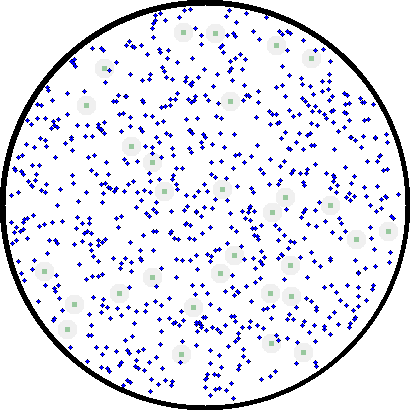
\includegraphics[width=2.5in]{robocoop/wander_env.png}
        \vskip 0.25cm
        \caption{The environment. Each blue dot is a robot. Each green dot is a resource and the light green circle around it is the patch. Robots can see the resources, and when two robots walk on a patch, they can interact together.
        }
    \label{fig:env}
    \end{center}
\end{figure}

When two robots are on the same patch, they can choose to interact together and exploit the resource. First, each robot accesses the action that its partner intends to do, then it decides whether or not to accept the interaction. If one of the robots choose not to interact, then the resource disappears and the robots continue their course. If both robots accept, the resource disappears and they play the announced investments to get their payoffs. The robots switch then to a wandering behaviour for a certain period of time. It represents the amount of time the robots interact with each other, or a digestion period. Each robot has a probability $\tau$ of returning to the game at each iteration. The expected duration of an interaction for an agent is therefore $1/\tau$. Two robots that have interacted together may not come back to partner seeking behaviour at the same iteration. When a resource disappears, a new resource appears in the arena at the next iteration.

\subsection{Cooperation Market} \label{sec:market}
According to the theoretical results on partner choice \citep{Debove2015b}, the efficiency of this strategy depends on the meeting probability of an agent ($\beta$) and the split probability of an interaction ($\tau$). If the meeting probability is big compared to the split probability, that is $\beta/\tau$ is large, then partner choice is a viable strategy and can emerge. Indeed, for partner choice to be effective, when an agent refuses to interact with a partner, it must do so because its expectation of gain in finding a better partner outweighs the gain missed by rejecting the interaction with the wrong partner and the implied cost paid by looking for a new partner. Thus, if search time is short compared to interaction time, it is profitable to spend more time searching for a good partner than interacting with more uncooperative partners.

The $\beta$ parameter is determined by the ability of the robots to meet on a patch and varies as the robots evolve, but also depending on the density of robots in the arena, and especially the robots that are also seeking for partner. In our model, the split probability $\tau$ parameter is chosen experimentally.

\subsection{Objective function}

When two robots interact with each other, they earn a gain determined by the investment of the two agents. The gain of an agent $a_i$ investing $x_i$ with its partner $a_j$ investing $x_j$ is determined by the function $P(x_i, x_j)$ described in the equation~\ref{eq:payoff}.

\begin{align}
PG(x_i, x_j) &= \frac{a}{2} (x_i + x_j) \\
PD(x_j) &= \frac{b}{2} (x_j) \\
C(x_i) &= \frac{1}{2} x_i^2 \\
P(x_i, x_j)& = PG(x_i, x_j) + PD(x_j) - C(x_i) \label{eq:payoff}
\end{align}

This function is a mixture of a public good ($PG$, modulated by $a$) and a prisoner's dilemma ($PD$, modulated by $b$) and a quadratic cost $C$. For $a_i$ to maximize its individual gain ($P(x_i, x_j)$), the optimal investment is $x_d = \frac{a}{2}$, which correspond to the defective behaviour. For the group to maximize their total gain, both agents must invest $\hat{x} = a + \frac{b}{2}$, which correspond to the cooperative behaviour. The Figure~\ref{fig:payoff} is a plot of the payoff function with different partner's investment values.



\begin{figure}[htpb]
    \centering
    \includegraphics[width=\columnwidth]{robocoop/payoff.pdf}
    \caption{Payoff function with different partner's investment value. The individually optimal investment is $x_d = \frac{a}{2}$ whatever the constant value the partner invests, which correspond to a defective behaviour. If both robots invest the same value, then the socially optimal investment is $\hat{x} = a + \frac{b}{2}$, which correspond to a cooperative behaviour.}
    \label{fig:payoff}
\end{figure}

\subsection{Controller}

The robot control system is composed of the investment value ($x \in [0, 10]$) during interaction and two decision modules: The movement module and the partner choice module. The robot always invests the same value and the modules remain fixed throughout the task. 

The movement module is an artificial neural network with 1 hidden layer of 10 neurons. All the nodes have a $\tanh$ activation function. The input of the network is the detailed information from the 8 sensors of the robot. The network gives as output the speed of translation and rotation between $]-1, 1[$. These values are then resized to match the maximum translation and rotation speeds of the robot.

The partner choice module is also a artificial neural network. It is activated only when an agent is with another agent on the same patch. This network receives as inputs the investment level of the robot as well as the investment level of its partner. It is composed of 1 hidden layer of 3 neurons and has a $\tanh$ activation function. It gives as output a value ($a \in ]-1, 1[$), which correspond to the response to the partner. If the output is greater than 0, then the robot accepts the interaction, otherwise it refuses it and the interaction does not take place.  The details of the inputs of each network are given in the Table~\ref{tab:ann_params}.

All neural network weights are bounded in the range $]-10, 10[$. In total, the two neural networks consist of 368 weights.

\begin{table}
    \centering
    \begin{tabular}{cc}
        \hline
        \textbf{Input} & \textbf{Value}  \\
        \hline
        \textbf{Movement module} & \\
        \textit{Per sensor ($\times 8$)}& \\
        Distance to Robot &  $]0, 1[$ if in range else 1 \\
        Distance to Wall & $]0, 1[$ if in range else 1  \\
        Distance to Resource & $]0, 1[$ if in range else 1  \\
        Robot on the patch & 0 or 1 \\
        \hline
        \textbf{Partner choice module} & \\
        Partner's investment & $]0, 10[$ \\
        Robot's own investment & $]0, 10[$ \\
        \hline
    \end{tabular}
    \caption{Neural Networks inputs}
    \label{tab:ann_params}
\end{table}

\subsection{Phenotypic variability} \label{sec:phenovar}

\citet{McNamara2010c} reviews different works that have shown the importance of variability in the level of investment in the population to allow agents' selectivity and thus enable the appearance of partner choice. Indeed, for selectivity to be a useful skill, the variability of investments between agents must be big enough so that the payoff variation between two different partners is sufficiently beneficial. In this case, selective robots have the upper hand against undiscriminating robots.

This variability can be present by itself or enforced either with a very high mutation strength for the gene encoding the investment level for each agent, or by adding a noise to the genetically encoded investment level for each agent that will remain the same throughout the task. 

\subsection{Learning}

The weights of the neural networks and the investment value of a robot constitute its genome. In total, a robot has $369$ genes, the $g_x$ gene to encode the investment level and the 368 $g_{w_i}\,\forall i \in 0..368$ genes to encode the weights of the two neural networks. The value of $g_x$ is in $]0, 1[$, the investment level $x$ of the robot is defined by $x = 10 \times g_x$. The values of $g_{w_i}$ are in $]-10, 10[$.

At the beginning of learning, the $g_{w_i}$ genes are randomly initialized in the range $]-1, 1[$ and the $g_x$ gene is randomly initialized in $]0, 1[$.

We use the fitness-proportionate evolutionary algorithm described below for the learning of our robots. After each generation, the total payoffs of the agents represent their fitnesses. Thus, the fitness $F_i$ of the robot $i$  which had accepted $n$ interactions is described by (Eq.~\ref{eq:totalpayoff})


\begin{equation}
    F_i = \frac{1}{\tau} \sum_{j=0}^{n} P(x_i, x_j) \label{eq:totalpayoff}
\end{equation}  

with $x_j$ being the investment value of the robot's partner at the $j^{th}$ interaction. Each payoff is weighted by $\tau$ to normalize the total payoff gains by robots between conditions where $\tau$ varies.

A new generation of robots is generated by randomly drawing the agents' genomes in proportion to their fitnesses. Then a mutation operation is applied to each agent of the new generation. Each $g_i$ gene of a robot has a probability $\mu = 0.01$ to mutate. If the gene is selected, then it has a probability of $0.1$ to mutate according to a uniform distribution $\mathcal{U}(]-10, 10[)$ and a probability of $0.9$ to mutate according to a normal distribution $\mathcal{N}(g_i, \sigma)$ with $\sigma = \sigma_w = 0.1$ for the weight genes and $\sigma = \sigma_x = 0.1$ for the investment gene. The new generation then performs the task and the process is repeated for $G = 200$ generations (see Table~\ref{tab:env_params} for a list of all the parameters). 

\begin{table}
    \centering
    \begin{tabular}{clc}
        \hline
        \textbf{Param} & \textbf{Description}  & \textbf{Value} \\
        \hline
        \multicolumn{3}{l}{\textbf{Payoff}} \\
        $a$ & Public good weight & 5 \\
        $b$ & Prisoner's dilemma weight & 3 \\
        %\hline
        \multicolumn{3}{l}{\textbf{Environment}} \\
        $T$ & Number of iterations per generation & $100\,000$ \\
        $G$ & Number of generations per run & $200$ \\
        & Arena diameter & 400px \\
        & Robot size & 4px \\
        & Robot max speed & 2px/iteration \\
        $\omega$ & Number of patches & 30 \\
        $\tau$ & End of interaction probability & \\
        %\hline
        \multicolumn{3}{l}{\textbf{Evolution hyper-parameters}} \\
        $\mu$ & mutation probability & 0.01 \\
        $\sigma_w$ & mutation strength of weight genes & 0.1 \\
        $\sigma_x$ & mutation strength of investment gene& 0.1 \\
        \hline
    \end{tabular}
    \caption{Experiment parameters}
    \label{tab:env_params}
\end{table}

\section{Results}

\subsection{Experimental setup}

The environment is a circular arena with a diameter of 400px. The robots are 4px diameter disks. The robots have 8 equally distributed sensors with a range of 96px giving them information about their surroundings, such as the presence of other robots, of a resource or of a wall. The robots move through the environment at a maximum translation speed of 2px/iteration and a rotational speed of $30^\circ$/iteration. $N$ robots are spread randomly in the environment and 30 resources are randomly scattered throughout the arena. Each generation lasts $T = 100\,000$ iterations. The environment is represented in Figure~\ref{fig:env}.

The results presented below are obtained by the behavioral study of the $200^{th}$ generation.  We ran 24 simulations per condition in all experiments.

We have studied the influence of several factors that may facilitate the emergence of partner choice and cooperation behaviours: (i) the effect of population size (ii) the effect of the duration of interactions by changing the split probability ($\tau$), and (iii) the strength of the investment gene mutation ($\sigma_x$). 

\subsection{Effect of the population size}

We first wanted to test the impact of the population size on the emergence of partner choice. Does a bigger population size positively impact the emergence of cooperative behavior? %question
To test the emergence of the cooperation behavior by partner choice, we set the parameters to be the most favourable for its emergence. We set $\tau = 0$ and the evaluation duration $T = 100\,000$ in order to grant a long search time for the robots and a very engaging commitment if they accept the interaction. %expe
At $N = 50$, robots plays the defective strategy. the average investment level is very close to the social optimum for $N = 1\,000$ (see Figure~\ref{fig:do_coop}). % results 
The robots evolve a cooperative behavior for $N$ sufficiently large. The denser the population, the higher the probability of encounters $\beta$ is. Thus, with 50 robots in the arena, the robots are unable to meet and sample enough partners to be selective before the end of the generation. Moreover, the robots are racing to find a partner quickly. Indeed, with $\tau = 0$, the more the task advances in time, the fewer agents are available in the arena and thus the more $\beta$ decreases throughout the evaluation. % interpretation



\begin{figure}[tbhp]
    \begin{center}
        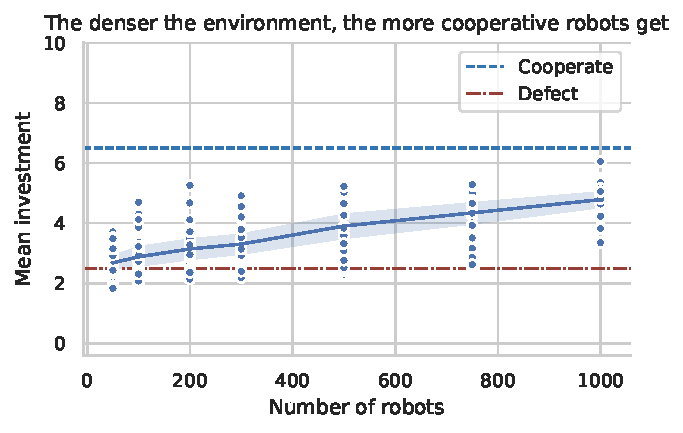
\includegraphics[width=3in]{robocoop/wander_do_coop.pdf}
        \vskip 0.25cm
        \caption{The larger the population, the higher the agents' level of investment.
        Mean investment of the population for 24 simulations per condition with a split probability $\tau = 0$ and a mutation strength for investment $\sigma_x = 0.1$. When the population is large, agents can easily find a partner and can be more selective. The pressure to invest a lot is then greater due to the effect of the partner choice.
        }
        \label{fig:do_coop}
    \end{center}
\end{figure}


To show the importance of partner choice in the evolution of this cooperative behavior, %question
we built a control condition where we deactivate the agents' ability to know their partner's investment in order to accept or not accept an interaction. % expe
In this condition, whatever the number of agents in the environment, the average investment level is always $x_d$, that is a defective behaviour (see Fig.~\ref{fig:control}). % results
In this situation, agents have no way to be selective and cannot choose a cooperative robot over a non-cooperative one. Thus, cooperative robots are not preferentially selected as partners and there is no incentive to invest more than the individual optimum. There is no selection pressure in favor of the most cooperative agents. % interpretation

\begin{figure}[tbhp]
    \begin{center}
        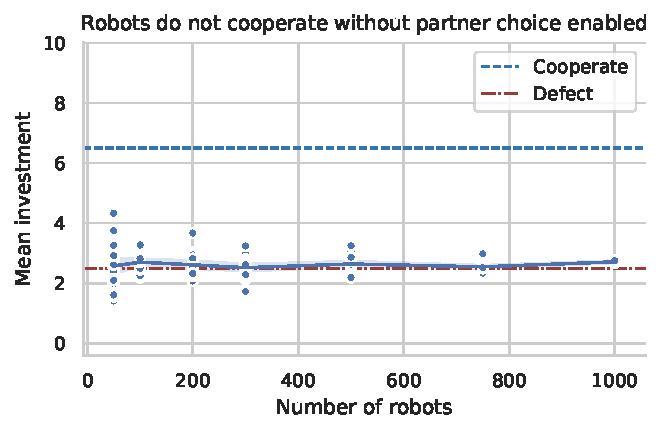
\includegraphics[width=3in]{robocoop/wander_control.pdf}
        \vskip 0.25cm
        \caption{Robots never cooperate in control condition. Mean investment of the population for 24 simulations per condition with a split probability $\tau = 0$ and a mutation strength of investment $\sigma_x = 0.1$. Robots never cooperate whatever the number of robots $N$ in the environment. Without access to their potential partner's investment level, agents cannot be selective and partner selection is impossible. Agents are under no pressure to invest a lot to be chosen. Therefore, they all play at the individually optimal investment level.
        }
        \label{fig:control}
    \end{center}
\end{figure}


\subsection{Effect of the interaction length}

%question
%expe
%results
%interpretation

According to the theoretical results, the longer the interaction, the greater the influence of the choice of partner (see section~\nameref{sec:market}). We test the reality of this prediction in our experimental setup. % question
To do this, we vary the split probability $\tau$.  % expe
The larger $\tau$ is, the shorter the interaction. When the split probability $\tau$ is null or low and the population size $N$ is large, the robots invest in a collectively optimal way and have a cooperative behavior (see Fig.~\ref{fig:corr_tau_comp}. % results
The larger the $\tau$ becomes, the less cooperative the robots are even for a high population size. The robots plays systematically a defective investment with $\tau \geq 1\times 10^{-3}$ Thus, increasing the duration of interactions has a positive effect on the appearance of cooperative behavior by partner choice. % interpretation


\begin{figure}[tbhp]
    \begin{center}
        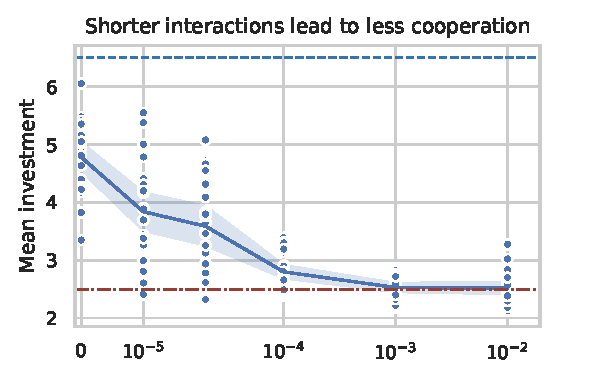
\includegraphics[width=3.3in]{robocoop/wander_corr_tau_coop_pop1000.pdf}
        \vskip 0.25cm
        \caption{The smaller the split probability $\tau$ is, the more cooperative robots get. The robots invest cooperatively for $\tau \leq 2\times 10 ^{-5}$, and have a defective behaviour for $\tau > 2 \times 10^{-5}$. The higher $\tau$ is, the less long are the interaction and the more profitable it is to interact with a lot of bad partner compared to looking for a good partner and interact with it.
        }
        \label{fig:corr_tau_comp}
    \end{center}
\end{figure}


\subsection{Effect of the mutation strength}

As explained in the section \nameref{sec:phenovar}, different works have shown the importance of variability in the level of investment in the population to allow agents' selectivity and thus enable the appearance of partner choice \citep{McNamara2010c}.
We test the influence of higher phenotypic variability in our task. % Question
To do so, we (i) modified the strength $\sigma_x$ of the Gaussian mutation on the gene encoding the robot investment level and (ii) applied a constant noise on the robot investment level during a generation. % expe
We observe very minor differences in the average investment level between the different simulations (see Fig~\ref{fig:varmut}). However, we note the presence of less variability between simulations when the mutation level is high. This can be explained by a more rapid convergence towards the optimal investment level. % resultats
The fact that the variability of investment in the environment plays very little role in our task may be explained by the fact that all possible levels of investment are present in the first generation. The ability to be selective in the choice of partner may therefore emerge before the population is completely homogeneous and thus selectivity becomes an unnecessary skill. % interpretation


\begin{figure}[tbhp]
    \begin{center}
        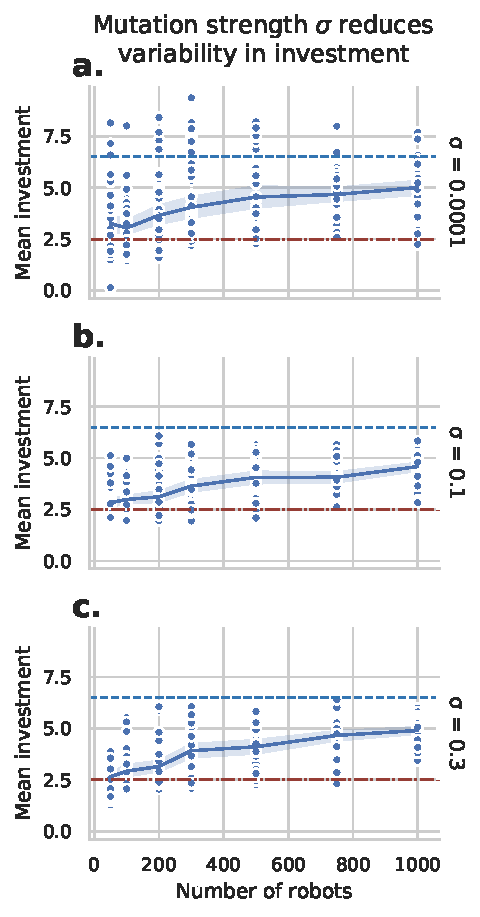
\includegraphics[width=2.4in]{robocoop/wander_varmut.pdf}
        \vskip 0.25cm
        \caption{A higher mutation strength has no impact on average cooperation but reduces variance in investment between simulations.
        Average investment in the population for 24 simulations per condition with $\tau = 0$. The addition of phenotypic variability facilitates the appearance of agent selectivity at low investment mutation strength \citep{McNamara2010c}. Here, variations in mutation strength for investment $\sigma_x$ %or the addition of phenotypic variability
        have only a small impact on the final investment level of the agents. This may be due to the fact that all possible investment levels are represented at the Initialization of the simulation.
        }
    \label{fig:varmut}
    \end{center}
\end{figure}



\subsection{Control: population size vs number of generations}

The difference in population size between low (50 robots) and high (1000 robots) population conditions could be explained by the lower number of evaluations that the 50 robot conditions have to evolve cooperative behaviour. Indeed, with the number of generations being constant ($G = 200$), the number of evaluations for the condition with 50 robots is $50 \times 200 = $10,000 and for the conditions with 1000 robots is $1,000 \times 200 = 200,000$. This difference in the number of evaluations could explain why cooperative behaviour has evolved in the conditions where $N$ is large and not in those where $N$ is small. Has the evolution converged in the small $N$ conditions? % Question
To test the impact of this number of evaluations, we run a new control condition of 24 simulations with $G = 4,000$ for a population of $N=50$ robots, offering $200\,000$ evaluations. % Method
The difference between the condition $N=50, G=200$ and $N=50, G=4000$ is marginal, but the difference between these conditions at the condition $N=1\,000, G=200$ is very large (Fig.~\ref{fig:gencomp}). Adding more generations does not improve the level of cooperation achieved for conditions with a small population. % results
It is therefore the too low encounter probability $\beta$ that blocks the emergence of cooperative behavior under these conditions, not the fewer evaluations. % interpretation


\begin{figure}[tbhp]
    \begin{center}
        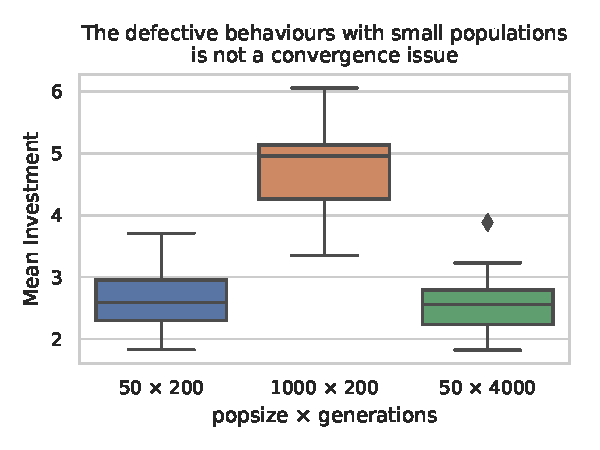
\includegraphics[width=3.3in]{robocoop/wander_comp_genpop.pdf}
        \vskip 0.25cm
        \caption{More generations with small population does not lead to cooperative behaviour. The differences in robot investment between conditions $N=50$ and $N=1000$ cannot be attributed to fewer evaluations for small populations.
        }
        \label{fig:gencomp}
    \end{center}
\end{figure}


\subsection{Control: Wandering vs Teleportation}


Finally, we do a final control to test the influence of the wandering behaviour. Does this facilitate or not the emergence of cooperation by partner choice? % Question
To test this, we compare the task with digestion time by wandering with a task with digestion time outside the arena. In this second condition, after one robot has interacted with another, it is placed outside the arena and has a $\tau$ probability of returning to the arena at each time step. When a robot is placed back into the arena, it is randomly placed back into the arena. This second condition is closer to the numerical simulations present in \citet{Debove2015c} than the wandering condition. We compare the results with the wandering condition and the condition outside the arena for several values of split probability $\tau$. % 2) Expe
We find that in the wandering condition as well as in the off-arena condition, when the probability of split is low ($\tau < 1\times 10^{-5}$), the robots invest cooperatively. We also find that in the off-arena condition, the robots remain cooperative for higher values of split probability. For even higher split probabilities, the robots no longer have cooperative behaviors whatever the condition. % results
The off-arena condition is more robust than the wander condition. Indeed, for higher split probability values, the agents still behave cooperatively. This can be explained by the fact that the arena is less crowded than in the wander condition. Indeed, a robot necessarily crosses potential partners in the off-arena condition, and is not blocked by agents in their digestion phase, as would be the case in the wander condition. Thus, the $\beta$ encounter probability is greater in the off-arena condition than in the wander condition. % 4) interpretation

\begin{figure}[tbhp]
    \begin{center}
        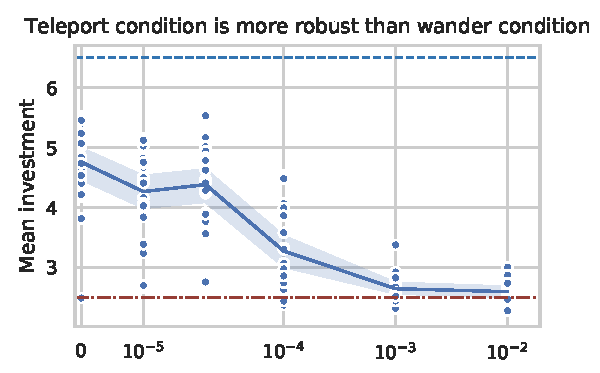
\includegraphics[width=3.3in]{robocoop/wander_corr_tau_coop_pop1000_tp.pdf}
        \vskip 0.25cm
        \caption{Robots act cooperatively in both the wander and off-arena conditions for low split probability $\tau$. The off-arena condition is more robust to middle range values of $\tau$ than the wander condition.
        }
        \label{fig:comp_tau_wander_tp}
    \end{center}
\end{figure}



\chapter{Discussion}
\input{chapters/05Discussion}

\printbibliography


\end{document}